\question{Термоэлектронная эмиссия. Уравнение Ричардсона-Дэшмана}
Термоэлектронной эмиссией называется процесс испускания электронов с поверхности
вещества, обусловленный нагревом.

Для того, чтобы электрон покинул поверхность металла и ушёл на бесконечность для
составляющей его скорости, нормальной к поверхности металла, должно выполняться
соотношение
\[
    \frac{mv_n^2}{2} \ge A,
\]
где в правой части стоит работа выхода из металла.
\begin{figure}[h]
\begin{center}
    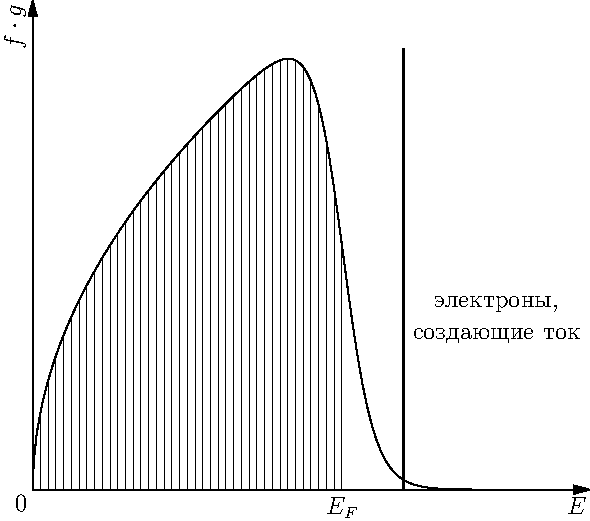
\includegraphics[width=.47\textwidth]{01}
\end{center}
\caption{Плотность состояний}
\end{figure}

Для определения числа электронов, пересекающих поверхность металла в единицу
времени, найдём распределение электронов по скоростям.
Из соотношения неопределённостей найдём объём ячейки фазового пространства:
\[
    \Delta x \Delta y \Delta z \Delta p_x \Delta p_y \Delta p_z \ge h^3.
\]
Пусть объём образца \( V \), тогда объём квантового состояния в пространстве
скоростей
\[
     \Delta v_x \Delta v_y \Delta v_z \ge \frac{h^3}{m^3V}.
\]
Так как электрон -- фермион, он подчиняется статистике Ферми-Дирака, и в каждой
квантовой ячейке может находиться 2 электрона. Поэтому, число электронов в
единице объёма имеющих скорость в кубике со сторонами \( dv_x, dv_y, dv_z \)
равно
\[
    dn = \frac{m^3}{h^3}\frac{2}{\exp\left[\left(\frac{mv^2}{2} -
    \mu\right)/kT\right]+1} dv_xdv_ydv_z.
\]
Плотность тока термоэлектронной эмиссии есть \( nev_x \), откуда
\[
    j = \int ev_x dn = \frac{2m^3e}{h^3}\exp\left(\frac{E_F}{kT} \right)
    \int_{v_{min}}^\infty v_x\exp\left(-\frac{mv_x^2}{2kT}\right)dv_x
    \int_{-\infty}^{+\infty}\int_{-\infty}^{+\infty}
    \exp\left(-\frac{m(v_y^2+v_z^2)}{2kT}\right)dv_ydv_z.
\]
Проинтегрировав, получаем уравнение Ричардсона-Дэшмана:
\[
    j = \frac{4\pi me k^2T^2}{h^3}
    \exp\left(-\frac{\frac{mv_{min}^2}{2} - E_F}{kT}\right) =
    CT^2\exp\left(-\frac{A}{kT} \right).
\]

